\section{Results}
    In this section, we will present the results of all three experiments. In the heatmaps, the by red enclosed cells indicates the environments from the testing set used for extrapolation testing, while the non-red-enclosed cells represent the environments from the training set used for interpolation testing. Lastly, we will present the results on the different types of morphologies evolved in our experiments.
    \subsection{Experiment 1: One generalist}
        \begin{figure*}[ht]
            \centering
            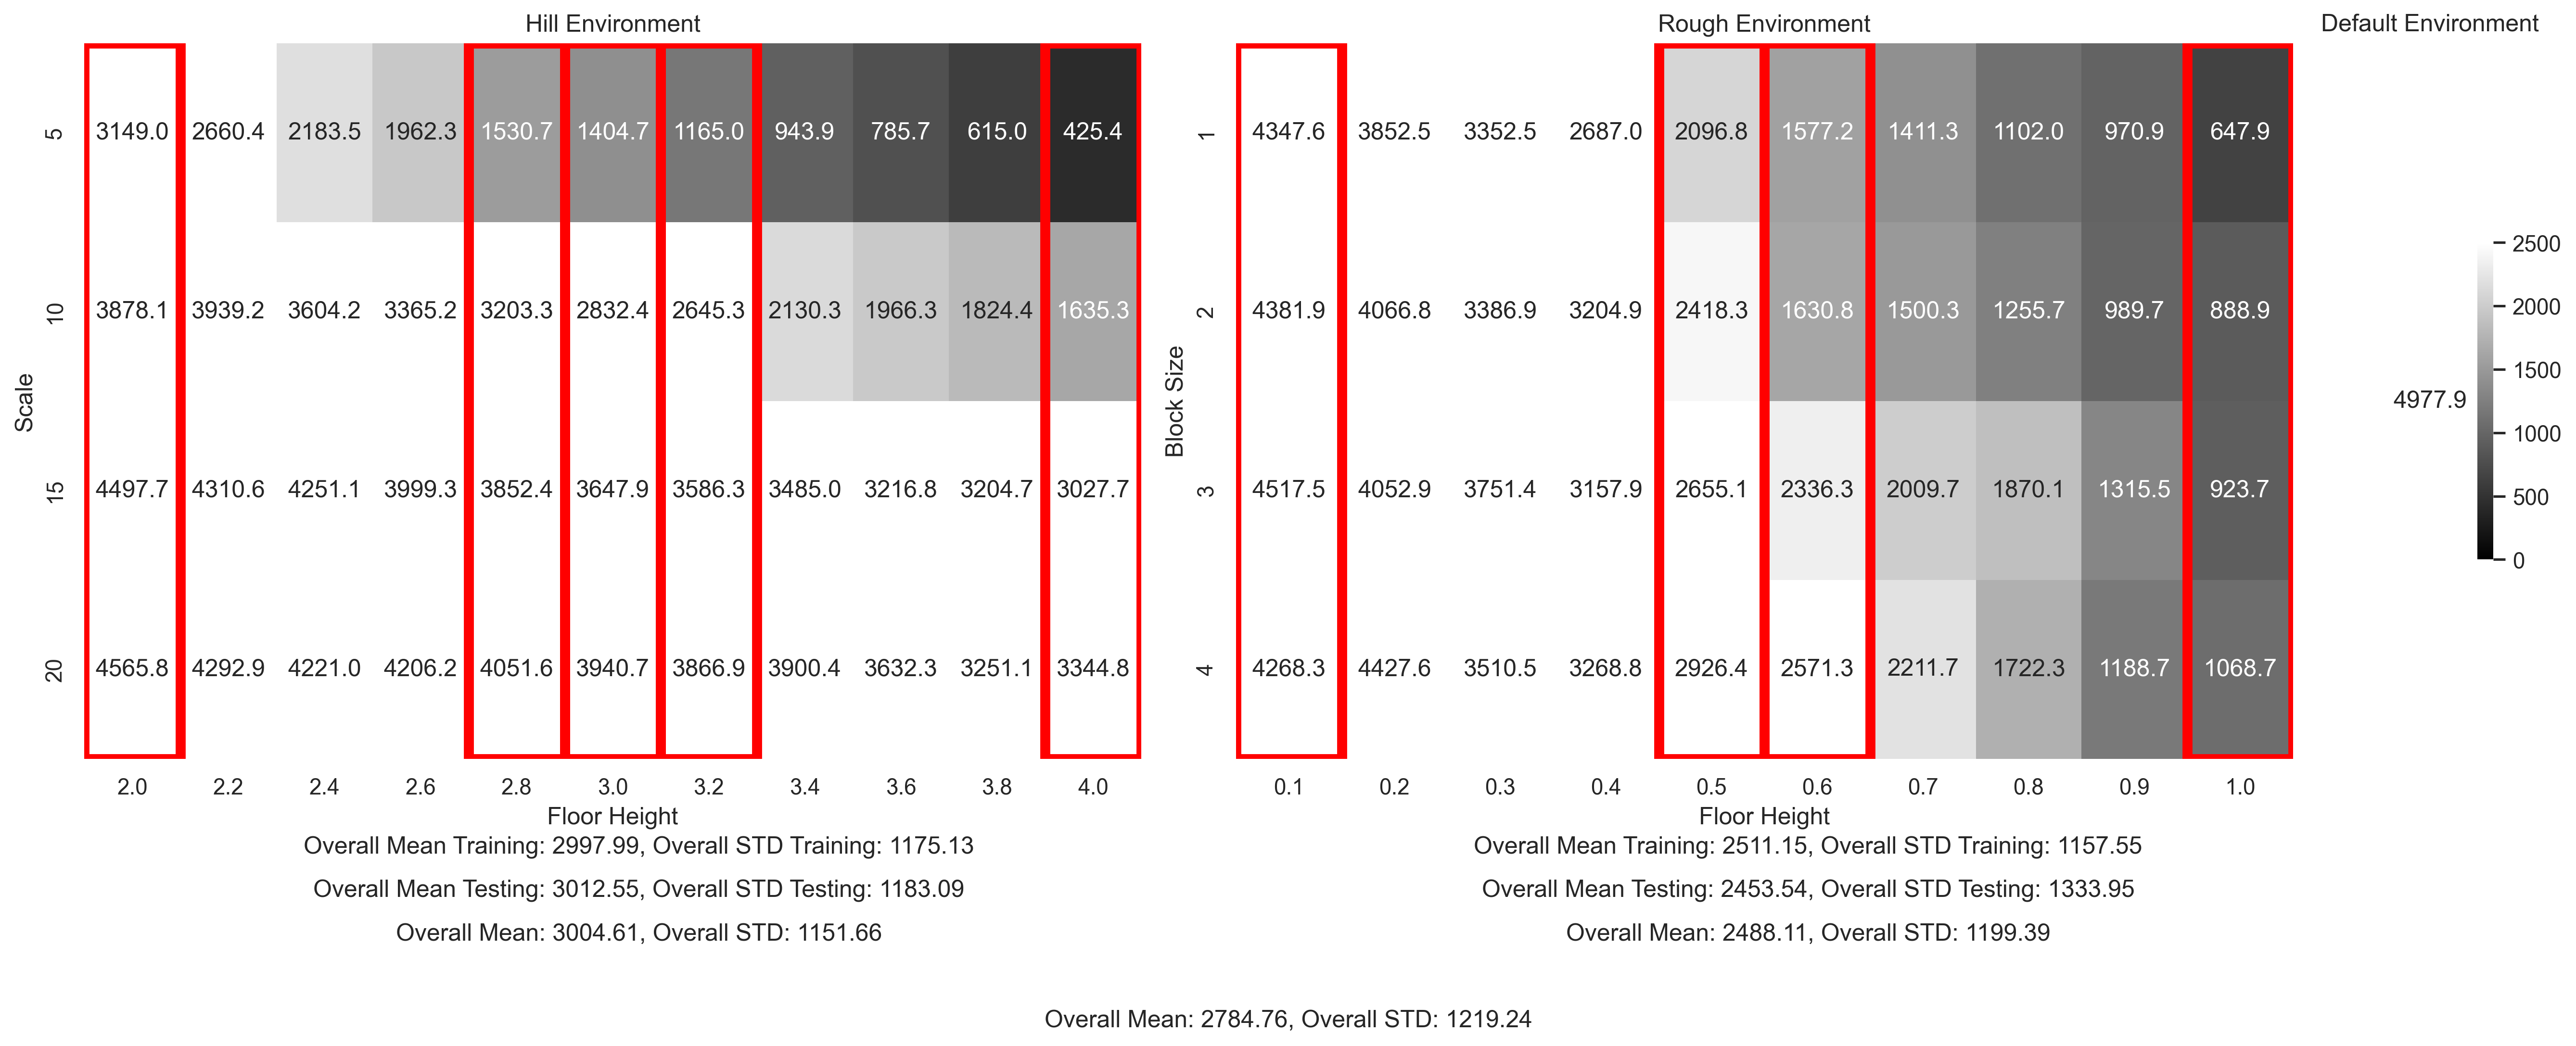
\includegraphics[width=\linewidth]{./resources/generalist_4_2784/fitness_heatmap.png}
            \caption{Experiment 1 - Fitness heatmap from one generalist MC-pair evolved over 5000 generations with partitions disabled}
            \label{fig:fit_heat_generalist}
        \end{figure*}

        Figure~\ref{fig:fit_heat_generalist} shows the obtained fitness scores for each environment, represented in a heatmap for experiment 1. For the hill environment, the heatmap shows high performance in the environments at the lower left and relatively lower performance when nearing the the upper right. This may indicate inherint complexity in certain environments compared to others. The fitness scores and their standard deviations on the training and testing sets are similar. The training set has a mean fitness score of 2997.99 with a standard deviation of 1175.13, and the testing set has a mean fitness score of 3012.55 with a standard deviation of 1183.09. 
        
        For rough terrain environment, the heatmap also shows high performance in the environments at the lower left and relatively lower performance when nearing the upper right, but also more at the lower right part. The fitness scores and their standard deviations on the training and testing sets are also similar. The training set has a mean fitness score of 2511.15 with a standard deviation of 1157.55, and the testing set has a mean fitness score of 2453.54 with a standard deviation of 1333.95.
    
        \subsection{Experiment 2: Partitioned generalist}
            \begin{figure*}[ht]
                \centering
                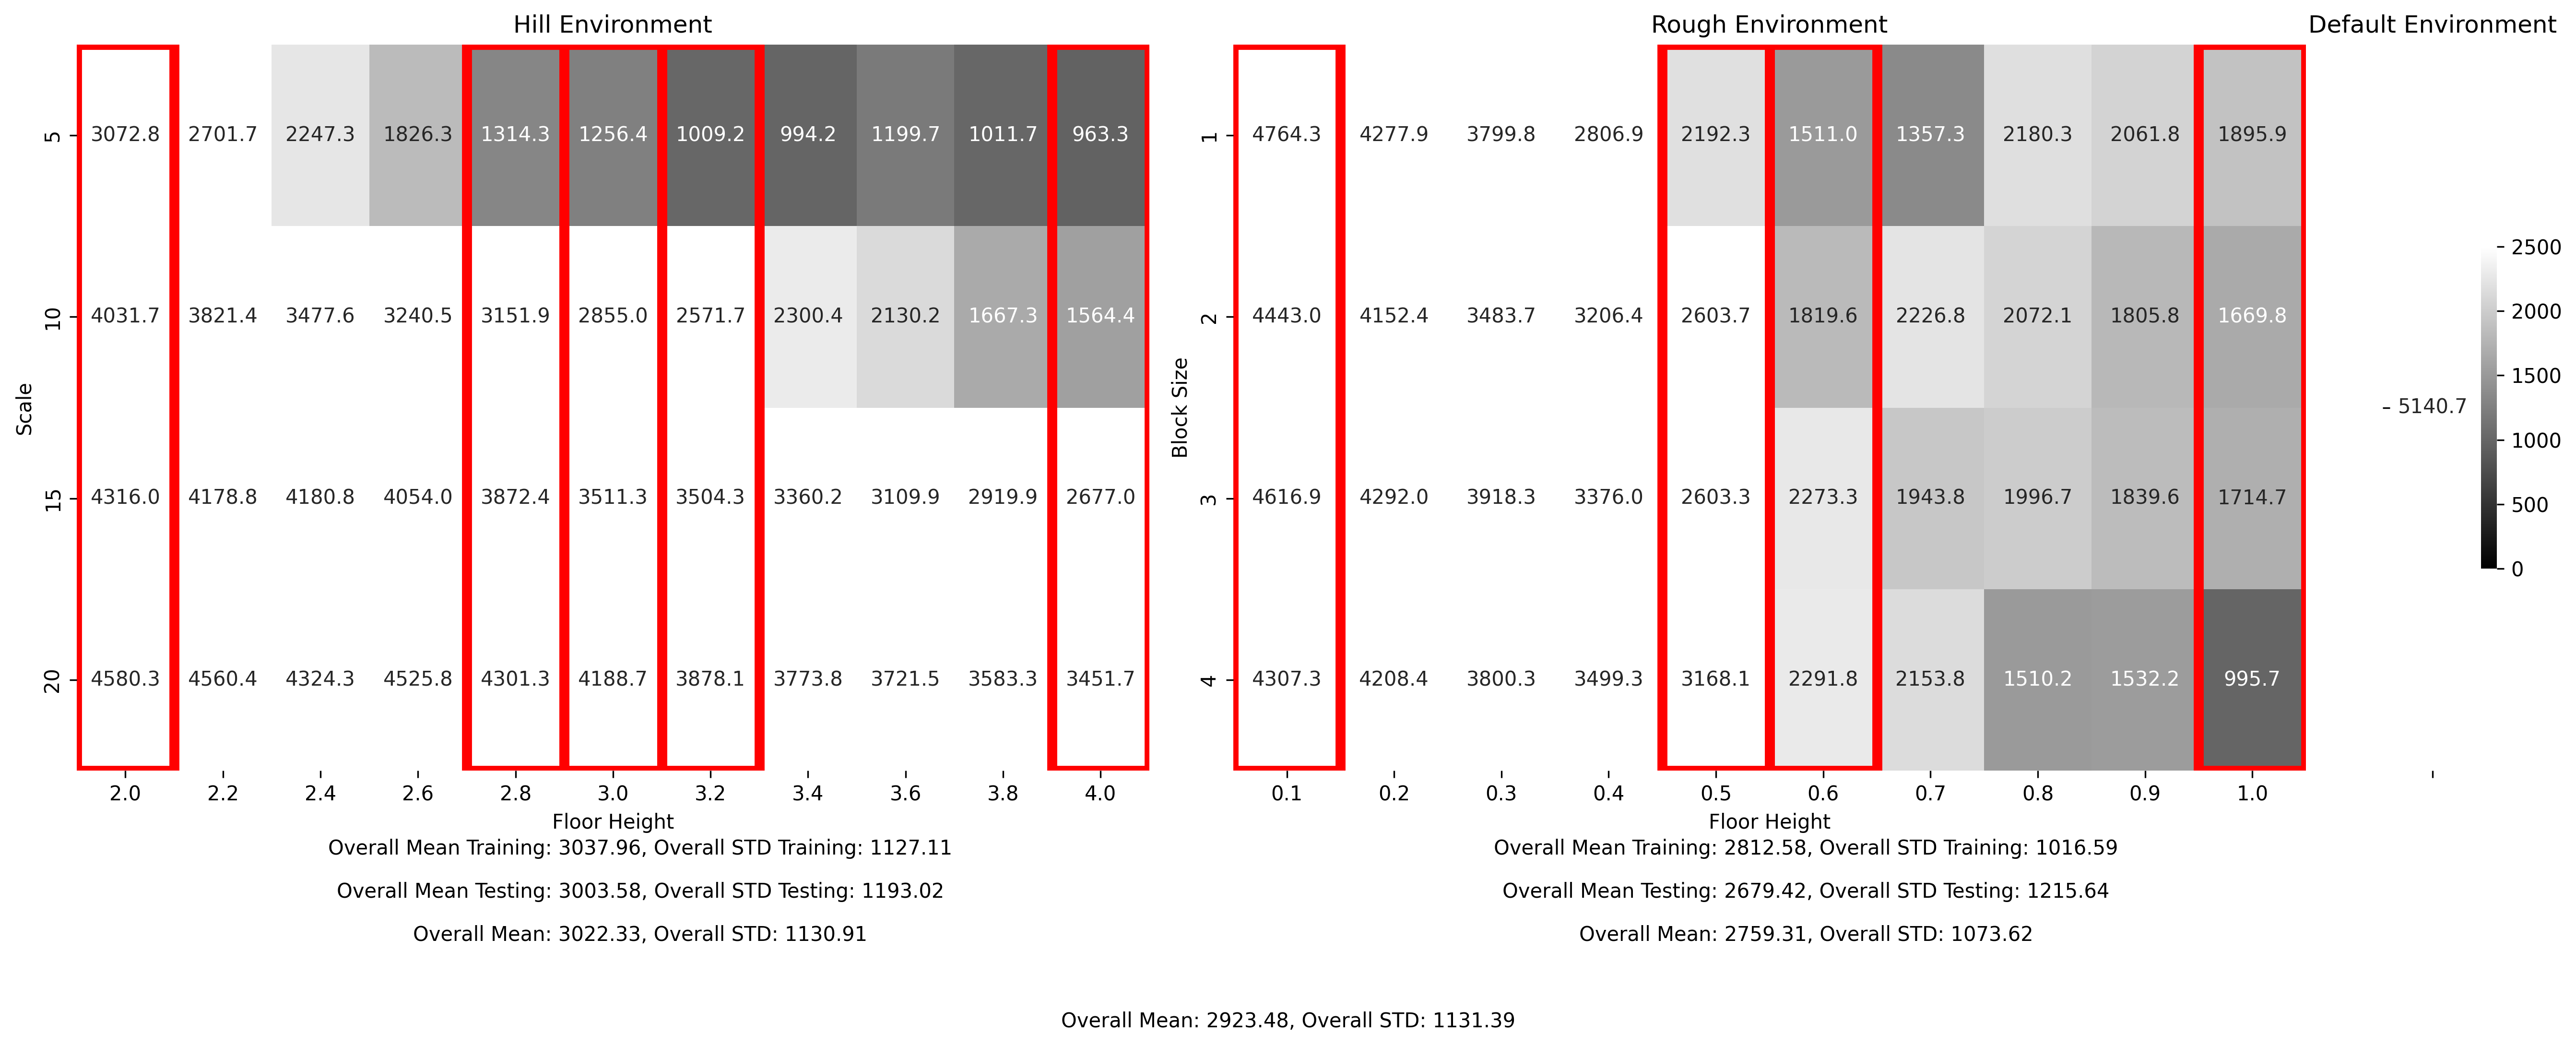
\includegraphics[width=\linewidth]{./resources/partition_5_2906_3/fitness_heatmap.png}
                \caption{Experiment 2 - Fitness heatmap of an ensamble of generalist MC-pair}
                \label{fig:fit_heat_partitioned}
            \end{figure*}

            Figure~\ref{fig:fit_heat_partitioned} shows the obtained fitness scores for each environment, represented in a heatmap for experiment 2. Similar to experiment 1, the hill environment shows high performance in the environments at the lower left, with relatively lower performance near the upper right. The fitness scores and their standard deviations for the training and testing sets are also similar. The training set has a mean fitness score of 3037.96 with a standard deviation of 1127.11, while the testing set has a mean fitness score of 3003.58 with a standard deviation of 1193.02. 

            For the rough terrain environment, the heatmap also shows high performance in the environments at the lower left and relatively lower performance near the upper right, and also in the lower right part, similar to experiment 1. The fitness scores on the training and testing sets are slightly different. The training set has a mean fitness score of 2812.58 with a standard deviation of 1016.59, and the testing set has a mean fitness score of 2679.42 with a standard deviation of 1215.64. 
            
            \begin{figure*}[ht]
                \centering
                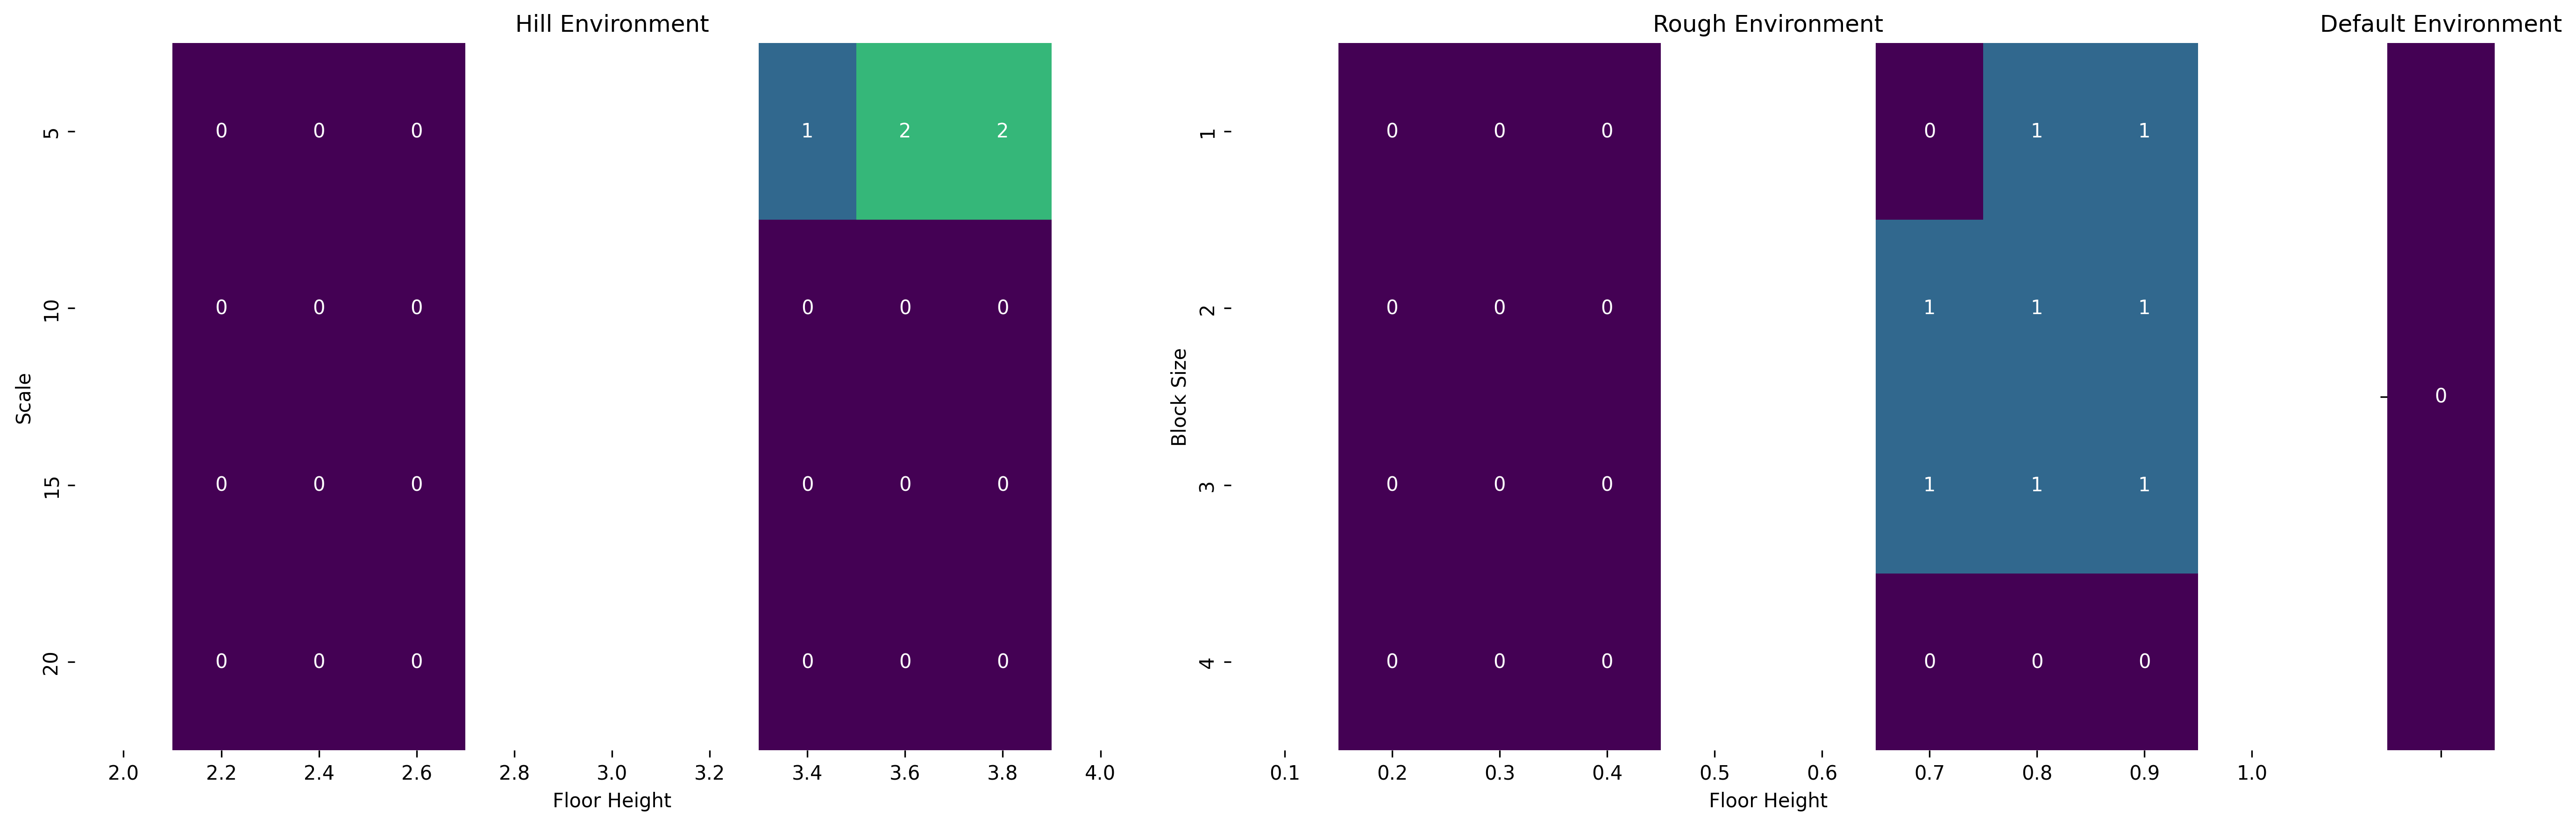
\includegraphics[width=\linewidth]{./resources/partition_5_2906_3/generalist_heatmap_partition.png}
                \caption{Experiment 2 - Figure showing to which partition the environment belongs to. In this experiment, three partitions where created.}
                \label{fig:heat_partition_number}
            \end{figure*}

            Overall, the ensamble MC-pairs do score a higher fitness on the rough terrain environment compared to experiment 1. This is evident when examining the partitions shown in figure~\ref{fig:heat_partition_number}. This figure presents the partitions to which each environment is assigned to. The blank white areas represent the testing environments that are not assigned to any partition. In this experiment, the environments in partition 1 and 2, that are being managed by another MC-pair, are of higher fitness scores, than in experiment one.

        \subsection{Experiment 3: Specialist for each environment}
            \textbf{Show similar visuals for Experiment 3}
        \subsection{Morphology}
            \begin{figure*}[ht]
                \centering
                \subfloat[2350]{%
                    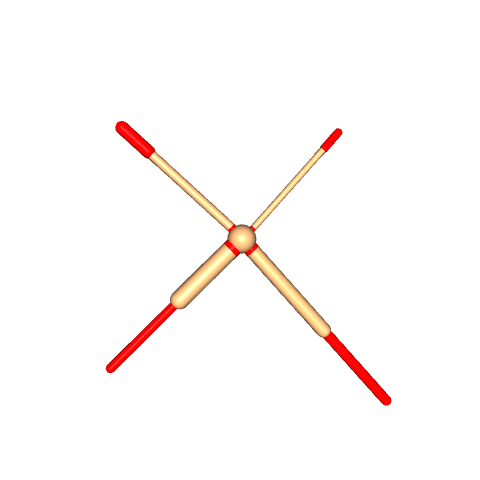
\includegraphics[width=0.2\linewidth]{resources/generalist_2_2350/ant.png}%
                    \label{fig:gen_ant_0}%
                }
                \hfill
                \subfloat[2412]{%
                    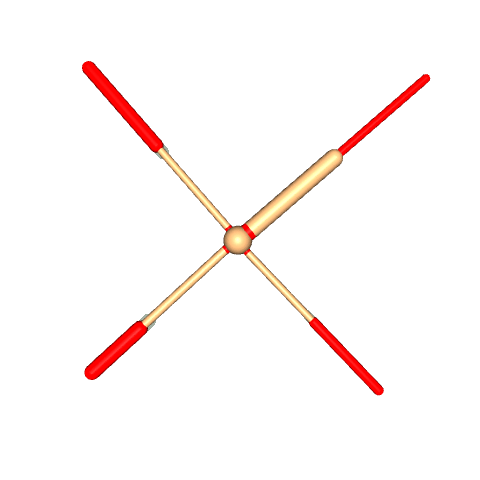
\includegraphics[width=0.2\linewidth]{resources/generalist_3_2412/ant.png}%
                    \label{fig:gen_ant_1}%
                }
                \hfill
                \subfloat[2784]{%
                    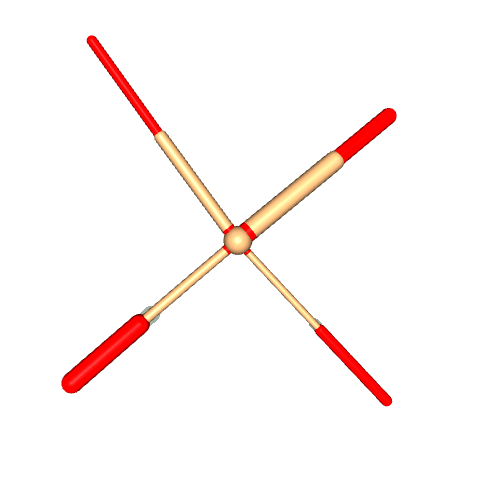
\includegraphics[width=0.2\linewidth]{resources/generalist_4_2784/ant.png}%
                    \label{fig:gen_ant_2}%
                }
                \hfill
                \subfloat[2966]{%
                    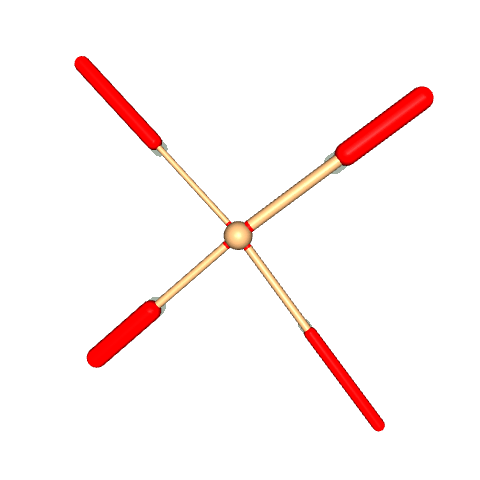
\includegraphics[width=0.2\linewidth]{resources/generalist_1_2966/ant.png}%
                    \label{fig:gen_ant_3}%
                }
                \hfill
                \subfloat[3126]{%
                    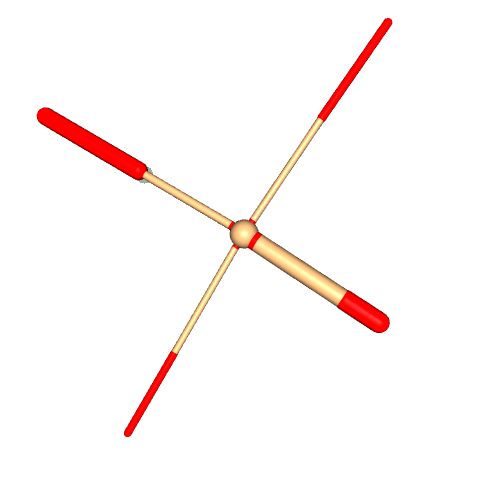
\includegraphics[width=0.2\linewidth]{resources/generalist_5_3126/ant.png}%
                    \label{fig:gen_ant_4}%
                }
                \caption{Experiment 1 - Morphology evolved for one generalist MC-pair from different evolutionary runs ordered by generalist score, which is shown below the image.}
                \label{fig:gen_ant_images}
            \end{figure*}
            A significant factor that determined the fitness score and the strategy utilized to achieve this score was the evolved morphology. Visualizations of these evolved MC-pairs from our different experiments can be viewed online\footnote{See the visual demonstration of the behaviors of the MC-pairs at: \url{http://site.com}}. In experiment 1, we conducted a total of five evolutionary runs, and the resulting MC-pairs are visible in Figure~\ref{fig:gen_ant_images}. These images are ordered by the generalist score obtained, which is shown below each image. The ants depicted in Figures~\ref{fig:gen_ant_1}, \ref{fig:gen_ant_2}, and \ref{fig:gen_ant_4} have similar morphological structures and employed very similar strategies to move forward, using its two side legs accellerate itself forward. In contrast, the ant in Figure~\ref{fig:gen_ant_3} uses a more conventional strategy, resembling more of how an actual ant would move.

            \begin{figure}[ht]
                \centering
                \subfloat[Partition 0]{%
                    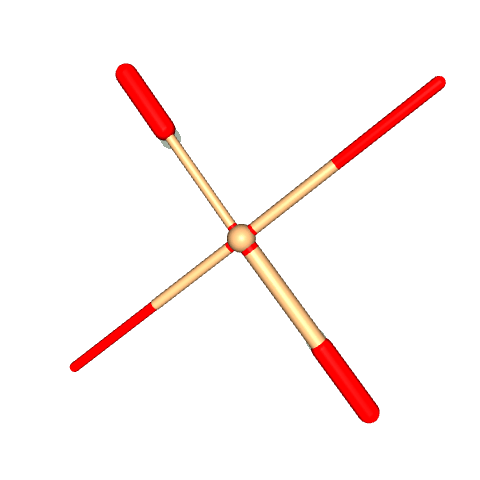
\includegraphics[width=0.3\linewidth]{resources/partition_5_2906_3/ant_0.png}%
                    \label{fig:part_ant_0}%
                }
                \hfill
                \subfloat[Partition 1]{%
                    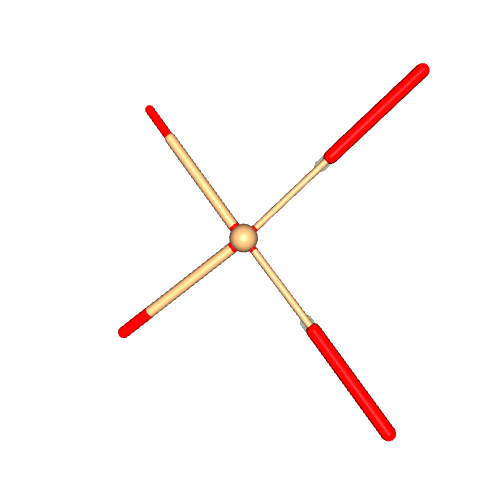
\includegraphics[width=0.3\linewidth]{resources/partition_5_2906_3/ant_1.png}%
                    \label{fig:part_ant_1}%
                }
                \hfill
                \subfloat[Partition 2]{%
                    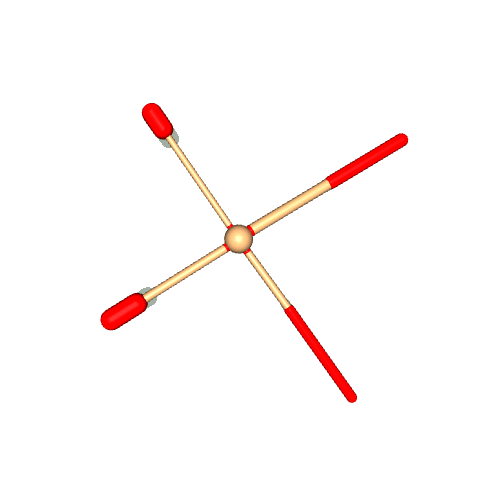
\includegraphics[width=0.3\linewidth]{resources/partition_5_2906_3/ant_2.png}%
                    \label{fig:part_ant_2}%
                }
                \caption{Experiment 2 - Morphology evolved for each partition}
                \label{fig:part_ant_images}
            \end{figure}
            In experiment 2, we have three different MC-pairs for three partitions, visible in Figure~\ref{fig:gen_ant_images}. The morphology in Figure~\ref{fig:part_ant_0} is similar to the morphologies from experiment 1 in Figures~\ref{fig:gen_ant_1}, \ref{fig:gen_ant_2}, and \ref{fig:gen_ant_4}. It also employs the same strategy to traverse the environment. This makes sense considering that experiment 1 is similar to the second experiment before partitioning. The morphology in Figure~\ref{fig:part_ant_1} has two long front legs and two short back legs, where the back legs were used to propel itself, over the terrain. Lastly, the morphology in Figure~\ref{fig:part_ant_2} is comparatively smaller, featuring two back legs with thicker lower portions. It uses its front legs to latch onto a elevated terrain and subsequently try to climb it by then hooking its back legs to climb.

            \textbf{Describe the novelties of the specialist controllers: Experiment 3}


